%%%%%%%%%%%%%%%%%%%%%%%%%%%%%%%%%%%%%%%%%%%%%%%%%%%%%%%%%%%%%%%%%%%
%                                                                 %
%   MINUIT - Reference Manual -- LaTeX Source                     %
%                                                                 %
%   Front Material: Title page,                                   %
%                   Copyright Notice                              %
%                   Preliminary Remarks                           %
%                   Table of Contents                             %
%   EPS file      : cern15.eps, cnastit.eps                       %
%                                                                 %
%   Editor: Michel Goossens / CN-AS                               %
%   Last Mod.:  18 Aug 1998                                       %
%                                                                 %
%%%%%%%%%%%%%%%%%%%%%%%%%%%%%%%%%%%%%%%%%%%%%%%%%%%%%%%%%%%%%%%%%%%

%%%%%%%%%%%%%%%%%%%%%%%%%%%%%%%%%%%%%%%%%%%%%%%%%%%%%%%%%%%%%%%%%%%%
%    Tile page                                                     %
%%%%%%%%%%%%%%%%%%%%%%%%%%%%%%%%%%%%%%%%%%%%%%%%%%%%%%%%%%%%%%%%%%%%
%begin{latexonly}
\def\Ptitle#1{\special{ps: /Printstring (#1) def}
                       \epsfbox{cnastit.eps}}
\begin{titlepage}
\vspace*{-23mm}
\includegraphics[height=30mm]{cern15.eps}%
\hfill
\raisebox{8mm}{\Large\bf CERN Program Library Long Writeup D506}
\hfill\mbox{}
\begin{center}
\mbox{}\\[10mm]
\mbox{\Ptitle{MINUIT}}\\[1cm]
{\Large Function Minimization and Error Analysis}\\[1cm]
{\LARGE Reference Manual}\\[2cm]
{\LARGE Version 94.1}\\[3cm]
{\Large F. James }\\[1cm]
{\Large Computing and Networks Division}\\[2cm]
\end{center}
\vfill
\begin{center}\Large CERN Geneva, Switzerland\end{center}
\end{titlepage}
%end{latexonly}
\begin{htmlonly}
\begin{center}{\Large\bf CERN Program Library Long Writeup D506}\\[5mm]
{\Huge MINUIT}\\[5mm]
{\Large Function Minimization and Error Analysis}\\[5mm]
{\LARGE Reference Manual}\\[5mm]
{\LARGE Version 94.1}\\[5mm]
{\Large F. James }\\[5mm]
{\Large Computing and Networks Division}\\[5mm]
{\Large CERN Geneva, Switzerland}\\[5mm]
\end{center}

\begin{rawhtml}
<HR>
<H3><A href="http://wwwinfo.cern.ch/asd/cernlib/minuit/minuit.ps">
PostScript version of this manual</A></H3>
<HR>
\end{rawhtml}
\end{htmlonly}



%%%%%%%%%%%%%%%%%%%%%%%%%%%%%%%%%%%%%%%%%%%%%%%%%%%%%%%%%%%%%%%%%%%%
%    Copyright  page                                               %
%%%%%%%%%%%%%%%%%%%%%%%%%%%%%%%%%%%%%%%%%%%%%%%%%%%%%%%%%%%%%%%%%%%%
\begin{htmlonly}
\chapter{Copyright Notice}
\end{htmlonly}
%begin{latexonly}
\thispagestyle{empty}
\framebox[\textwidth][t]{\hfill\begin{minipage}{0.96\textwidth}%
\vspace*{3mm}
\begin{center}Copyright Notice\end{center}
\parskip\baselineskip
%end{latexonly}
{\bf MINUIT -- Function Minimization and Error Analysis}
\par 
CERN Program Library entry {\bf D506}
\par
\copyright{} Copyright CERN, Geneva 1994--1998
\par
Copyright and any other appropriate legal protection of these
computer programs and associated documentation reserved in all
countries of the world.
\par
These programs or documentation may not be reproduced by any
method without prior written consent of the Director-General
of CERN or his delegate.
\par
Permission for the usage of any programs described herein is
granted apriori to those scientific institutes associated with
the CERN experimental program or with whom CERN has concluded
a scientific collaboration agreement.
\par
Requests for information should be addressed to:
%begin{latexonly}
\vspace*{-.5\baselineskip}
\begin{center}
\tt\begin{tabular}{l}
CERN Program Library Office              \\
CERN-IT Division                         \\
CH-1211 Geneva 23                        \\
Switzerland                              \\
Tel.      +41 22 767 4951                \\
Fax.      +41 22 767 8630                \\
Internet: cernlib@cern.ch                
\end{tabular}
\end{center}
\vspace*{2mm}
\end{minipage}\hfill}%end of minipage in framebox
\vspace{6mm}
%end{latexonly}
\begin{htmlonly}
\par
\begin{flushleft}
CERN Program Library Office              \\
CERN-IT Division                         \\
CH-1211 Geneva 23                        \\
Switzerland                              \\
Tel.: +41 22 767 4951                    \\
Fax.: +41 22 767 8630                    \\
Internet: \texttt{cernlib@cern.ch}                
\end{flushleft}
\par
\end{htmlonly}

%begin{latexonly}
{\bf Trademark notice: All trademarks appearing in this guide are acknowledged as such.}
\vfill
\begin{tabular}{l@{\quad}l@{\quad}>{\tt}l}
\emph{Contact Person}:           & Ian McLaren     /IT &(Ian.Mclaren\atsign cern.ch)\\[1mm]
\emph{Cocumentation consultant}: & Michel Goossens /CN &(goossens\atsign cern.ch)\\[1cm]
{\em Edition -- August 1998}
\end{tabular}
%end{latexonly}
\begin{htmlonly}
{\bf Trademark notice: All trademarks appearing in this guide are acknowledged as such.}

\begin{tabular}{lll}
\emph{Contact Person}:           & Ian McLaren /IT     & \texttt{Ian.Mclaren@cern.ch}\\
\emph{Documentation consultant}: & Michel Goossens /IT & \texttt{goossens@cern.ch}\\
\emph{Edition -- August 1998}
\end{tabular}
\end{htmlonly}
\newpage
 
%%%%%%%%%%%%%%%%%%%%%%%%%%%%%%%%%%%%%%%%%%%%%%%%%%%%%%%%%%%%%%%%%%%%
%    Introductory material                                         %
%%%%%%%%%%%%%%%%%%%%%%%%%%%%%%%%%%%%%%%%%%%%%%%%%%%%%%%%%%%%%%%%%%%%
%begin{latexonly}
\pagenumbering{roman}
\setcounter{page}{1}

\chapter*{Foreword}

\section*{What Minuit is intended to do.}
%end{latexonly}
\begin{htmlonly}
\chapter{Foreword}
\subsection*{What Minuit is intended to do.}
\end{htmlonly}
Minuit is conceived as a tool to find the minimum value of a
multi-parameter function and analyze the shape of the function around
the minimum. The principal application is foreseen for statistical
analysis, working on chisquare or log-likelihood functions, to compute
the best-fit parameter values and uncertainties, including
correlations between the parameters.  It is especially suited to
handle difficult problems, including those which may require guidance
in order to find the correct solution.
%begin{latexonly}
\section*{What Minuit is not intended to do.}
%end{latexonly}
\begin{htmlonly}
\subsection*{What Minuit is not intended to do.}
\end{htmlonly}

Although Minuit will of course solve easy problems faster than complicated
ones, it is not intended for the repeated solution of identically parametrized
problems (such as track fitting in a detector) where a specialized
program will in general be much more efficient.
 
%begin{latexonly}

\section*{Further remarks.}
 
In this manual examples are in {\tt monotype face} and strings to be
input by the user are {\tt\underline{underlined}}.  In the index the
page where a routine is defined is in {\bf bold}, page numbers where a
routine is referenced are in normal type.  In the description of the
routines a \texttt{*} following the name of a parameter indicates that
this is an {\bf output} parameter.  If another \texttt{*} precedes a
parameter in the calling sequence, the parameter in question is both
an {\bf input} and {\bf output} parameter.

This document has been produced using \LaTeX~\cite{bib-LATEX} with the
\texttt{cernman} style option, developed at CERN.  A compressed
PostScript file \texttt{minuit.ps.gz}, containing a complete printable
version of this manual, can be obtained from any CERN machine by
anonymous ftp as follows (commands to be typed by the user are
underlined):

\vspace*{3mm} 
\begin{alltt}\footnotesize
    \underline{ftp asis01.cern.ch}
    Trying 128.141.201.136...
    Connected to asis01.cern.ch.
    220 asis01 FTP server (Version 6.10 ...) ready.
    Name (asis01:username): \underline{anonymous}
    Password: \underline{your\_{}mailaddress}
    230 Guest login ok, access restrictions apply.
    ftp> \underline{cd cernlib/doc/ps.dir}
    ftp> \underline{get minuit.ps}
    ftp> \underline{quit}
\end{alltt}

%%%%%%%%%%%%%%%%%%%%%%%%%%%%%%%%%%%%%%%%%%%%%%%%%%%%%%%%%%%%%%%%%%%%
%    Tables of contents ...                                        %
%%%%%%%%%%%%%%%%%%%%%%%%%%%%%%%%%%%%%%%%%%%%%%%%%%%%%%%%%%%%%%%%%%%%

\newpage
\tableofcontents
%\newpage
\listoffigures
\listoftables
%end{latexonly}
